% Author: Seongjin Lee
% Hanyang University, Seoul, Korea
% esos.hanyang.ac.kr
% 2016-09-01
% note: some slides are adopted from  \url{www.cs.stevens.edu/~jschauma/631A/}
% https://github.com/resourceful/lecture_sysprog/

\documentclass[newPxFont,sthlmFooter,nooffset]{beamer}
\usepackage{kotex}
%\usetheme{sthlm}
\usepackage{../beamer_template/beamerthemesthlm}
\hypersetup{pdfauthor={Seongjin Lee (insight@gnu.ac.kr)},
            pdfsubject={Lecture Note: System Programming},
            pdfkeywords={Lecture Note, System Programming, class, (under)graduate},
            pdfmoddate={D: \pdfdate},
            pdfcreator={Seongjin Lee}}

%\setbeamertemplate{footline}[text line]{%
%    \parbox{\linewidth}{\vspace*{-8pt} \insertsectionhead  \hfill\insertshortauthor\hfill\insertpagenumber}}
%\setbeamertemplate{navigation symbols}{}



\title{System Programming}
\subtitle{Topic 1: Introduction to System Programming}
\author[SJL]{Seongjin Lee}
\institute{\href{mailto:insight@gnu.ac.kr}{insight@gnu.ac.kr}\\\url{http://open.gnu.ac.kr}\\Systems Research Lab.\\Gyeongsang National University}
\date{\today}

\begin{document}



\frame[plain]{\titlepage}

\begin{frame}[t]{Table of Contents}\vspace{2pt}

\begin{enumerate}
\item Nutshell
\item Introduction
\item History
\item Unix architecture
\item Logging in
\item Files and directories
\item Input and output
\item Programs and processes
\item Error handling
\item User Identification
\item Signals
\item Time values
\item System Calls and Library Functions
\item The Editors
\begin{enumerate}
      \item Vim
      \item Emacs
\end{enumerate}

\end{enumerate}

\end{frame}


%---------------------------------------------------------
\section{Nutshell}

\begin{frame}[t]{}
\begin{figure}\centering
  \includegraphicscopyright[width=0.7\linewidth]
   {./figure/ken-dennis-pdp7.jpg}
   {Ken Thompson and Dennis Ritchie at PDP-11 in 1971 (Photo: \href{https://www.bell-labs.com/usr/dmr/www/kd14.jpg}{Courtesy of Bell Labs)}}
\end{figure}

\end{frame}

\begin{frame}[t]{Principles}
\url{https://en.wikipedia.org/wiki/Unix_philosophy}
\bigskip
\begin{itemize}
\item Small is beautiful.
\item Make each program do one thing well.
\item Build a prototype as soon as possible.
\item Choose portability over efficiency.
\item Store data in flat text files.
\item Use software leverage to your advantage.
\item Use shell scripts to increase leverage and portability.
\item Avoid captive user interfaces.
\item Make every program a filter.
\end{itemize}
\end{frame}


\begin{frame}[t]{Introduction}
\begin{itemize}
 \item Familiarize with \textsc{Unix}
 \item Experience systems programming
 \item Understand fundamental OS concepts
  \begin{itemize}
    \item Multi-user concepts
    \item Basic and advanced I/O
    \item Process
    \item Interprocess communication
  \end{itemize}
\end{itemize}
\end{frame}



\begin{frame}[t]{Why do we have to?}
\begin{itemize}
 \item \textsc{Unix} gives you insights on how other OS works
 \item You can only catch the tiger by going into the tiger's den
 \item It is the basis for most other programming and understanding of the system
 \item It in C helps you understand the general programming concepts
\end{itemize}
\end{frame}


\begin{frame}[t]{How are we going to do?}
\lstinputlisting{./codes/welcome.c}

How to compile \\
\$ cc -Wall -g -o welcome welcome.c
\end{frame}


\begin{frame}[t]{About this class}
Textbook
\begin{itemize}
	\item ``Advanced Programming in the UNIX Environment'', by
		W. Richard Stevens, Stephen A. Rago (3rd Edition)
\end{itemize}
\bigskip
Assistant
\begin{itemize}
	\item Yeonjin Noh (\href{mailto:nyg0813@gmail.com }{nyg0813@gmail.com})
	\item FTC \#804
\end{itemize}
\bigskip


\bigskip
Grading:
\vspace{-1em}
\begin{multicols}{2}
\begin{itemize}
	\item Attendance 5$\%$
	\item Assignments 30$\%$
	\item Quiz 5$\%$
	\item Midterm Exam 30$\%$
	\item Final Exam 30$\%$
	\item Level test on editors
\end{itemize}
\end{multicols}
\end{frame}


\begin{frame}[t]{Syllabus}
\begin{columns}\small
\begin{column}{.48\linewidth}
\hangindent=1cm
Week 1 09-07 Introduction to system programming \& Shell Survival Kit
%\\•	Introduction, UNIX history, UNIX Programming Basics
%\\•	Working with Text Editor – Vi and Emacs (Level Test)
%\\•	Regular Expression

Week 2 09-14 (추석)

\hangindent=1cm
Week 3 09-21 Files IO \& ctag/etag
%\\•	File related operations
%\\•	Text editor with ctag/etag

\hangindent=1cm
Week 4 09-28 Files and Directories
%\\•	On struct stat
%\\•	Device special files
%\\•	Related operations

\hangindent=1cm
Week 5 10-05 Standard I/O Library
%\\•	Standard Input, output, and error
%\\•	Buffering
%\\•	Positioning a stream

\hangindent=1cm
Week 6 10-12 Process Environment
%\\•	Program Execution and Termination
%\\•	Memory Layout of a C program

Week 7 10-19 Process Control
%\\•	Process identifiers
%\\•	Process control operations

Week 8 10-26 (중간고사)
\end{column}

\begin{column}{.48\linewidth}
Week 9 11-02 Signals
%\\•	Concepts
%\\•	Interrupted system calls
%\\•	Related Functions

Week 10 11-09 Threads
%\\•	Thread concepts
%\\•	Creation and termination

Week 11 11-16 Thread Control
%\\•	Thread synchronization
%\\•	Locks

Week 12 11-23 Advanced I/O
%\\•	Non blocking I/O
%\\•	Memory mapped I/O

\hangindent=1cm
Week 13 11-30 Interprocess Communication I
%\\•	Pipes
%\\•	Message queues

\hangindent=1cm
Week 14 12-07 Interprocess Communication II
%\\•	Semaphores
%\\•	Shared memory

Week 15 12-14 Network IPC
%\\•	Vi and emacs (Level Test)
%\\•	Sockets
Week 16 12-21 (기말고사)
\end{column}
\end{columns}
\end{frame}



%---------------------------------------------------------
\section{History}
\begin{frame}[t]{The \textsc{Unix} History}
For more info :
\url{http://www.unix.org/what_is_unix/history_timeline.html}
\bigskip
\begin{itemize}
	\item Originally developed in 1969 at Bell Labs by Ken Thompson
		and Dennis Ritchie.
	\item 1973, Rewritten in C. This made it portable and changed the history of OS
	\item 1974: Thompson, Joy, Haley and students at Berkeley develop
		the {\bf B}erkeley {\bf S}oftware {\bf D}istribution (BSD) of UNIX
	\item two main directions emerge: BSD and what was to become ``System V''
\end{itemize}
\end{frame}

\begin{frame}[t]{\textsc{Unix} History}
\begin{itemize}\small
	\item 1984 4.2BSD released (TCP/IP)
	\item 1986 4.3BSD released (NFS)
	\item 1991 Linus Torvalds starts working on the Linux kernel
	\item 1993 Settlement of USL vs. BSDi; NetBSD, then FreeBSD are created
	\item 1994 Single UNIX Specification introduced
	\item 1995 4.4BSD-Lite Release 2 (last CSRG release); OpenBSD
		forked off NetBSD
	\item 2000 Darwin created (derived from NeXT, FreeBSD, NetBSD)
	\item 2003 Xen; SELinux
	\item 2005 Hadoop; DTrace; ZFS; Solaris Containers
	\item 2006 AWS ("Cloud Computing" comes full circle)
	\item 2007 iOS; KVM appears in Linux
	\item 2008 Android; Solaris open sourced as OpenSolaris
\end{itemize}

list from \url{www.cs.stevens.edu/~jschauma/631A/}

\end{frame}



\begin{frame}[c]{History}
\centering
\includegraphics[width=0.9\textwidth]{./figure/history_1.png}
\end{frame}


\begin{frame}[c]{History}
\centering
\includegraphics[width=0.9\textwidth]{./figure/history_2.png}
\end{frame}


\begin{frame}[t]{Some \textsc{Unix} Versions}
More UNIX (some generic, some trademark, some just unix-like):
\\
{
\fontsize{5pt}{6pt}\selectfont
\begin{tabular}{ c c c c c}
	1BSD & 2BSD & 3BSD & 4BSD & 4.4BSD Lite 1 \\
	4.4BSD Lite 2 & 386 BSD & A/UX & Acorn RISC iX & AIX \\
	AIX PS/2 & AIX/370 & AIX/6000 & AIX/ESA & AIX/RT \\
	AMiX & AOS Lite & AOS Reno & ArchBSD & ASV \\
	Atari Unix & BOS & BRL Unix & BSD Net/1 & BSD Net/2 \\
	BSD/386 & BSD/OS & CB Unix & Chorus & Chorus/MiX \\
	Coherent & CTIX & Darwin & Debian GNU/Hurd & DEC OSF/1 ACP \\
	Digital Unix & DragonFly BSD & Dynix & Dynix/ptx & ekkoBSD \\
	FreeBSD & GNU & GNU-Darwin & HPBSD & HP-UX \\
	HP-UX BLS & IBM AOS & IBM IX/370 & Interactive 386/ix & Interactive IS \\
	IRIX & Linux & Lites & LSX & Mac OS X \\
	Mac OS X Server & Mach & MERT & MicroBSD & Mini Unix \\
	Minix & Minix-VMD & MIPS OS & MirBSD & Mk Linux \\
	Monterey & more/BSD & mt Xinu & MVS/ESA OpenEdition & NetBSD \\
	NeXTSTEP & NonStop-UX & Open Desktop & Open UNIX & OpenBSD \\
	OpenServer & OPENSTEP & OS/390 OpenEdition & OS/390 Unix & OSF/1 \\
	PC/IX & Plan 9 & PWB & PWB/UNIX & QNX \\
	QNX RTOS & QNX/Neutrino & QUNIX & ReliantUnix & Rhapsody \\
	RISC iX & RT & SCO UNIX & SCO UnixWare & SCO Xenix \\
	SCO Xenix System V/386 & Security-Enhanced Linux & Sinix &
		Sinix ReliantUnix & Solaris \\
	SPIX & SunOS & Tru64 Unix & Trusted IRIX/B & Trusted Solaris \\
	Trusted Xenix & TS & UCLA Locus & UCLA Secure Unix & Ultrix \\
	Ultrix 32M & Ultrix-11 & Unicos & Unicos/mk & Unicox-max \\
	UNICS & UNIX 32V & UNIX Interactive & UNIX System III & UNIX System IV \\
	UNIX System V & UNIX System V Release 2 & UNIX System V Release 3 &
		UNIX System V Release 4 & UNIX System V/286 \\
	UNIX System V/386 & UNIX Time-Sharing System & UnixWare & UNSW & USG \\
	Venix & Wollogong & Xenix OS & Xinu & xMach \\
\end{tabular}
}
\bigskip

\hfill {\footnotesize adopted from \url{http://www.cs.stevens.edu/~jschauma/631A/}}
\end{frame}





%---------------------------------------------------------
\section{The \textsc{Unix} Basics}

\begin{frame}[t]{The \textsc{Unix} Basics: Architecture}
applications $>$ shell
\bigskip
~
\centering
\includegraphics[height=0.85\textheight]{./figure/System-Call-and-Library-Function.png}
\end{frame}



\begin{frame}[t]{UNIX Architecture}\vspace{4pt}
\textbf{Kernel} is a software (SW) that controls the hardware (HW) of the computer and provides an environment under which programs can run.

\textbf{System calls:} are entry points into which kernel codes where the functions are implemented.\\[6pt]
\textbf{Library calls (functios):} are transfers to user code with which performs the desired functions.

An \textbf{operating system (OS)} consists of the kernel and all other SWs that make a computer useful and gives the computer its personality. Other SW include system utilities, applications, shells, libraries of common functions etc. For example, for linux, kernel used by GNU OS is GNU(sometimes referred to as GNU linux OS) has an advantage of being more siccunt.

\end{frame}

\begin{frame}[t]{Logging In}\vspace{10pt}
After log in, the system looks up for your login in its password file (/etc/passwd) which is composed of 7 colon separated fields (login name, encrypted password, user ID 205), numeric group ID (105), a comment field, home directory (/home/sar) and shell program (/bin/ksh). That is, sar: x: 205: 105: Sembaty Erios: home/sar: /bin/ksh. (chapter 6).

\textbf{Shell:} is a command-line interpreter that reads user input and executes commands. It is a special application that provides an interface for running other applications.

After log in, you type commands to the shell and the system knows which shell to execute for us based on the field in our entry password file. 
\end{frame}

\begin{frame}[t]{Logging In}\vspace{10pt}
The system knows which shell to execute for us based on the final field in our entry in the password file.\\[10pt]\textbf{There are 5 common shells used} (chapter 2) as shown in Table 1.
\\[6pt]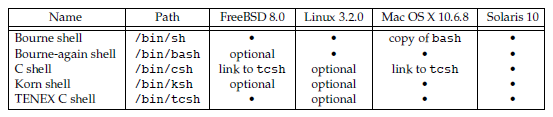
\includegraphics[scale=0.8]{shellstable.png}
Table 1: Showing common shells used on UNIX systems
\end{frame}

\begin{frame}[t]{Files and Directories}
\textbf{NOTE:} The research Unix system and some older Unix system v-file systems filenames are restricted to 14 characters. BSD versions – extended limit of 255 characters and almost all commercial Unix file systems support 255 character filenames.
\\[10pt]\textbf{Pathname:} is a sequence of 1 or more filenames separated by slashes (relative pathname) and starting with a slash (an absolute pathname). Relative pathname files are relative to the current directory.
\\[4pt]\textbf{Working directory:} every process has a working directory (current working directory) which interprets all relative pathnames. A process can change its directory with the chdir function.\\[10pt]
\textbf{Home directory:} after log in the working directory, it is set to our home directory which is obtained from our entry in the password.

\end{frame}

\begin{frame}[t]{Input and Output}
\textbf{File descriptors:} are small non-negative integers that the kernel uses to identify the files accessed by a process. Whenever the kernel opens an existing file or creates a new file, it returns a file descriptor that we use when we want to read or write a file.\\[6pt]
\textbf{Standard input, standard output and standard error:} usually, all shells provide a way to redirect and/or all the descriptors to any file. If nothing is done, like a simple command 1s, then all d 3 are connected to the terminal (chapter 18). For example; s>file.list executes the 1s command with its standard output redirected to the file named .file.list (chapter 5).

\end{frame}

\begin{frame}[t]{Programs and Processes}
\textbf{Program} is an executable file residing on disk in a directory. A program is read into memory and is executed by the kernel as a result of one of the seven exec functions (Section 8.10).\\[10pt]
\textbf{A process (task):} An executing instance of a program. 
The UNIX System guarantees that every process has a unique numeric identifier (is always a non-negative integer) called the \textbf{process ID}. 
\\[6pt]\textbf{Process Control:}  There are three primary functions for process control: fork, exec (has seven variants), and waitpid. Process control of UNIX system is demonstrated by the bare-bornes implementation of the shell-like program (chapter 8). 

\end{frame}

\begin{frame}[t]{Programs and Processes}
\subtitle{Threads and Threads ID}
\textbf{Threads:} A thread is a set of machine instructions executing at a time. A process usually has only 1 thread of control. Some problems are easy to solve when more than 1 thread of control operates on different parts of the problem. Multiple threads of control can exploit the parallelism possible on multiprocessor systems.
\\[6pt]All threads within a process share \textbf{the same address space, file descriptors, stacks and process-related attributes.} Each thread executes on its own stack but any thread can access stacks of other threads in the process. They need to synchronize access to share data amongst themselves to avoid inconsistent.
\\[4pt]\textbf{Thread ID:} It functions to control threads parallel to other threads used to control a process. Threads are localized to a process (chapter 12). A thread ID from one process has no meaning in another process. We use thread IDs to refer to specific threads as we manipulate the threads within a process.

\end{frame}

\begin{frame}[t]{Error Handling}
Occurrence of an error in UNIX system functions returns \textbf{a negative value and the integer errno} is usually set to a value that notifies you. Eg, open function returns either a non-negative file descriptor in all, to indicate all is ok or -1 for error. That is; more functions that return a pointer to an object, return a null pointer to indicate an error. An error from open has about 15 possible errno values, say, file does not exist, permission problem (section 2).
\\[6pt]On LINUX, the error constants are listed in the errno (3) manual page. In an environment that supports threads, the process address space is shared by amongst multiple threads with each thread having its own local copy of errno to prevent them from interfering with each other. 


\end{frame}

\begin{frame}[t]{Error Handling}
\textbf{There are 2 rules to be aware of with respect to errno.} 
\\[6pt]1. Its value is never cleared by a routine if an error does not occur. Thus, we should examine its value only when the return of errno is never set to 0 by any of the functions and no constants defined in errno.h has a 0 value.
\\[6pt]2. The value of errno is never set to 0 by any of the functions and none of the constants defined in <errno.h> has a value 0. 

\end{frame}

\begin{frame}[containsverbatim,t]{Error Handling: ANSI C}
\begin{itemize}
	\item	Important ANSI C Features:
		\begin{itemize}
			\item function prototypes
			\item generic pointers ({\tt void *})
			\item abstract data types (e.g. {\tt pid\_t}, {\tt size\_t})
		\end{itemize}
	\item	Error Handling:
		\begin{itemize}
			\item meaningful return values
			\item {\tt errno} variable
			\item look up constant error values via two functions:
		\end{itemize}
\end{itemize}

\begin{lstlisting}
#include <string.h>
char *strerror(int errnum) // returns pointer to message string
\end{lstlisting}

\bigskip

\begin{lstlisting}
#include <stdio.h>
void perror(const char *msg)
\end{lstlisting}

\end{frame}

\begin{frame}[t,fragile]{Errors and Warnings}
\begin{lstlisting}
$ gcc -Wall -g -o welcome welcome.c
welcome.c:6:81: warning: implicit declaration of function 'getlogin'
        is invalid in C99 [-Wimplicit-function-declaration]
        printf("Welcome to System Programming, %s!\n", getlogin())
                                                       ^
welcome.c:6:81: warning: format specifies type 'char *' but the
        argument has type 'int' [-Wformat]
        printf("Welcome to System Programming, %s!\n", getlogin())
                                               ~~      ^~~~~~~~~~
                                               %d
welcome.c:6:92: error: expected ';' after expression
        printf("Welcome to System Programming, %s!\n", getlogin())
                                                                  ^
                                                                  ;
2 warnings and 1 error generated.
\end{lstlisting}


\end{frame}


\begin{frame}[t]{Error Recovery}
\textbf{Fatal error} has no recovery action. It is where you only print an error message on the user ’s screen or to a log file, and then exit.\\[6pt]
\textbf{Nonfatal errors} are temporary, such as a resource shortage, and occur when there is less activity on the system. \\[6pt]\textbf{Resource-related nonfatal errors:-} EAGAIN, ENFILE, ENOBUFS, ENOLCK, ENOSPC, EWOULDBLOCK, and sometimes ENOMEM. EBUSY can be treated as nonfatal when it indicates that a shared resource is in use as well as EINTR when it interrupts a slow system call.\\[6pt]
\textbf{The recovery action for a resource-related nonfatal error} is to delay and retry later. Eg, network connection is no longer functioning.
Some applications use an exponential back off algorithm, which takes a long time in each subsequent iteration and is dependent on the developer.


\end{frame}


\begin{frame}[t]{User Identification (ID)}
The \textbf{user ID} from our entry in the password file is a numeric value that identifies us to the system. 
User whose user ID is 0 either root or the superuser. The entry in the password file normally has a login name of root and the special privileges of this user as superuser privileges (chapter 4).\\[6pt]
\textbf{Group ID:} here, the password file contains multiple entries specifying the same group ID. Groups are normally used to collect users together into projects or departments and allows sharing of resources, such as files, among members of the same group. 
The group file (/etc/group) maps group names into numeric group IDs. 

For every file on disk, the file system stores both the user ID and the group ID (which values requires only four bytes) of a file’s owner assuming that each is stored as a two-byte integer.

\end{frame}
\begin{frame}[t]{Supplementary Group ID}
These \textbf{supplementary group IDs} are obtained at login time by reading the file /etc/group and finding the first 16 entries that list the user as a member (chapter 2).\\[6pt]
Most versions of the UNIX System allow a user to belong to other groups (it started with 4.2BSD, at least 16 additional groups).


\end{frame}
\begin{frame}[t]{Signals}
Are a technique notifies a process that some condition has occurred. For example, if a process divides by zero, the signal whose name is SIGFPE (floating-point exception) is sent to the process (Chapter 10).
\\[6pt]The process has \textbf{3 choices for dealing with the signal;-} 
\\[6pt]1. Ignore the signal. Not recommended for signals that denote a hardware exception, such as dividing by zero or referencing memory outside the address space of the process, as the results are undefined.
\\[6pt]2. Let the default action occur. For a divide-by-zero condition, the default is to terminate the process.
\\[6pt]3. Provide a function that is called when the signal occurs \textbf{(called ‘‘catching’’ the signal)}. 


\end{frame}
\begin{frame}[t]{Signals}
\textbf{Interrupt key—}(DELETE key or Control-C —) and the \textbf{quit key—}(Control-backslash — ): used to interrupt the currently running process. Thus to generate a signal is by calling the kill function (from a process to send a signal to another process).\\[6pt]
\textbf{Limitations to call a function :} you must be the owner of the other process (or the superuser) to be able to send it a signal.


\end{frame}
\begin{frame}[t]{Time Values}
UNIX systems have \textbf{maintained two different time values:}
\textbf{Calendar time:} This value counts the number of seconds since the Epoch: 00:00:00 January 1, 1970, Coordinated Universal Time (UTC). (Older manuals refer to UTC as Greenwich Mean Time.) These time values are used to record the time when a file was last modified.
\\[6pt]\textbf{Process time (CPU time):} measures the central processor resources used by a process and is measured in clock ticks (have historically been 50, 60, or 100 ticks per second)\textbf{(section 2.5.4)}.

\end{frame}

\begin{frame}[t]{Time Values}
\textbf{Measurement of  the execution time of a process (Section 3.9):}
\\[4pt]UNIX System maintains three values for a process:
\\[6pt]\textbf{Clock time (wall clock time) -} amount of time the process takes to run, and its value depends on the number of other processes being run on the system and the measurements are made with no other activities on the system.
\\[3pt]\textbf{User CPU time -} CPU time attributed to user instructions, that is; attributed to the kernel when it executes on behalf of the process. 
\\[3pt]\textbf{System CPU time -} The sum of user CPU time and system CPU time is often called the CPU time.
\


\end{frame}
\begin{frame}[t]{Time Values}
\textbf{Measurement of the clock time, user time, and system time of any process:} simply execute the time(1) command, with the argument to the time command being the command we want to measure.\\[6pt]
\textbf{Note:} The output format from the time command depends on the shell being used, because some shells don’t run /usr/bin/time, but instead have a separate built-in function to measure the time it takes commands to run (Section 8.17).
\end{frame}

\begin{frame}[t]{System Calls and Library Functions}
An application can either make a system call or call a library routine but library routines invoke a system call \textbf{Figure 3.}

The exact number of system  calls varies depending on the operating system version (Section 2 of the UNIX Programmer ’s Manual defines the general-purpose library functions available to programmers). Linux 3.2.0 has 380 system calls and FreeBSD 8.0 has over 450. The technique used on UNIX systems is for each system call to have a function of the same name in the standard C library. The user process calls this function, using the standard C calling sequence.  Which invokes the appropriate kernel service. The exact number of system  calls varies depending on the operating system version \textbf{(check Section 2 of the UNIX Programmer’s Manual defines the general-purpose library functions available to programmers).} Eg, Linux 3.2.0 has 380 system calls and FreeBSD 8.0 has over 450. The technique used on UNIX systems is for each system call to have a function of the same name in the standard C library.

\end{frame}

\begin{frame}[t]{System Calls and Library Functions}
The user process calls this function, using the standard C calling sequence  which invokes the appropriate kernel service.
From \textbf{an implementer's point of view,} the distinction between a system call and a library function is fundamental. \textbf{For example; 1-} System calls usually provide a minimal interface while library functions often provide more elaborate functionality. \textbf{2-} System calls allocate additional chuck of space on behalf of the process wile library functions manage space from user level.
\\[4pt] Unlike \textbf{a user}, for the implementer, both system calls and library functions appear as normal C functions.  As both exist to provide services for application programs. We can replace the library functions whereas the system calls usually cannot be replaced.\\[4pt]
\textbf{Section 8.13 -} show an implementation of the system function that invokes the basic process control system calls with \textbf{an example in Section 10.18} to handle signals correctly.

\end{frame}



%---------------------------------------------------------
\section{The Editors}
\subsection{Vim}
\begin{frame}[t]{}
\begin{figure}\centering
  \includegraphicscopyright[width=\linewidth]
   {./figure/vi_why.png}
   {\centering Image from \url{http://michael-prokop.at/computer/tools_vim_en.html}}
\end{figure}
\end{frame}

\begin{frame}[t]{What is Vi(m)}
\textbf{Vi} is a visual screen text editor developed by Bill Joy, who later becomes co-founder of Sun Micro Systems
\begin{itemize}
\item It is visual version of \textbf{ex}, a Unix line editor
\item Vi is available on most Unix Systems
\item Works with a variety of terminals
\item Allows \textbf{ex} command from \textbf{vi}
\end{itemize}
\bigskip

\begin{center}
 \includegraphics[width=0.7\linewidth]{./figure/bill_joy_quotes.jpg}
\end{center}
\end{frame}


\begin{frame}[t]{What is Vim}
\begin{columns}
\begin{column}{0.8\linewidth}
\textbf{VIM} is acronym for \textbf{Vi} i\textbf{M}proved, developed by Bram Moolenaar, a extended version of vi and some of enhancements include
\begin{itemize}
\item Completion, comparison, and merging of files
\item Split and tabbed windows
\item Command histories
\end{itemize}
\bigskip
All editing session before saving is done in buffer area
\begin{itemize}
\item Nothing is saved as hard data, until you save it
\end{itemize}
\end{column}
\begin{column}{0.2\linewidth}
  \includegraphics[width=0.8\linewidth]{./figure/vim_logo.png}
\end{column}
\end{columns}
\end{frame}


\begin{frame}[t]{Modes of vi}
There are three mode in vi
\begin{itemize}
\item \textbf{Command Mode} – A default mode in vi
\begin{itemize}
\item Everything is command before you enter into other modes
\end{itemize}
\item \textbf{Input Mode} – What you type is what you see
\begin{itemize}
\item Anything typed in this mode is considered as data
\item Pressing [ESC] always leads to Command mode
\end{itemize}
\item \textbf{Last Line Mode} – Only can be accessed from Command mode
\begin{itemize}
\item Three ways to enter Last Line Mode – : (Colon) / (Back Slash) ? (Question Mark)
\end{itemize}
\end{itemize}
\begin{center}
 \includegraphics[width=0.8\linewidth]{./figure/vi_modes.png}
\end{center}
\end{frame}




\begin{frame}[t]{Moving Around}
VI uses four characters to move around, and each character is mapped to a direction

\begin{center}
 \includegraphics[width=0.7\linewidth]{./figure/vi_directions.png}
\end{center}

Moving by units of word, sentence, paragraph
\begin{itemize}
\item E.g., 3w moves to three words after the current cursor
\end{itemize}


\keystroke{w} next word \hfill \keystroke{b} previous word \hfill \keystroke{(} Beginning of sentence

\bigskip
\keystroke{)} end of sentence \hfill \keystroke{\{} Beginning of paragraph \hfill \keystroke{\}} end of paragraph
\end{frame}


\begin{frame}[t]{Deleting}
Deleting a character, words, sentence, line, and paragraph
\begin{itemize}
 \item \keystroke{x} erases a character
 \item Combination of direction commands with \keystroke{d} erases a word, sentence, and paragraph.
\begin{itemize}
\item E.g., \keystroke{dw} erases a word before the cursor
\end{itemize}
 \item \keystroke{dd} erases a line
 \item \keystroke{D} to delete rest of line
 \item \keystroke{X} to delete before the cursor
 \item \keystroke{Xp} to transpose
\end{itemize}

\end{frame}



\begin{frame}[t]{Searching and Replacing}
Searching in vi is done in last line mode
\begin{itemize}
\item \keystrokered{/} lets you search a character, word, and words
\begin{itemize}
\item E.g., \keystroke{/abc} moves the cursor to the location of the pattern
\end{itemize}
\item Search pattern in forward direction: \keystroke{n}, backward direction: keystroke{N}
\item Regular expressions can be also used in searching
\end{itemize}
\bigskip

\keystroke{r} replaces a character
\begin{itemize}
\item Suppose the cursor is on \keystroke{b}, and by \keystrokered{r} \keystroke{p} we can change it to “preview”
\end{itemize}
\begin{center}
\keystroke{breview} $\rightarrow$ \keystrokered{preview}
\end{center}

\end{frame}


\begin{frame}[t]{Substitution}
\begin{center}
\textbf{Substituting in vi is done in last line mode}
\end{center}
\bigskip
Find i and substitute with X once
\vspace{0.5em}
\begin{center}
\begin{tabular}{ p{1cm} c p{3cm} c p{3cm}}
\keystrokered{:s/i/X} & $\rightarrow$ & This is preview. How it is done & $\rightarrow$ & ThXs is preview. How it is done \\
\end{tabular}
\end{center}
\bigskip
Find i and substitute with X in the same line
\vspace{0.5em}
\begin{center}
\begin{tabular}{ p{1cm} c p{3cm} c p{3cm}}
\keystrokered{:s/i/X/g} & $\rightarrow$ & This is preview. How it is done & $\rightarrow$ & ThXs is prevXew. How it is done \\
\end{tabular}
\end{center}
\bigskip
Find i and substitute with X in all the lines
\vspace{0.5em}
\begin{center}
\begin{tabular}{ p{1cm} c p{3cm} c p{3cm}}
\keystrokered{:\%s/i/X/g} & $\rightarrow$ & This is preview. How it is done & $\rightarrow$ & ThXs is prevXew. How Xt Xs done \\
\end{tabular}
\end{center}
\end{frame}




\begin{frame}[t]{Undo and Redo}
Undo in vi is done by \keystroke{u}
\begin{itemize}
\item Or to do in last line mode you could type in \keystroke{:undo}
\item \keystroke{U} undo all latest changes on one line
\end{itemize}
\bigskip

Redo in vi is done by \keystroke{CTRL}\keystroke{R}
\begin{itemize}
\item Or to do in last line mode you could type in \keystroke{:redo}
\end{itemize}

\end{frame}



\begin{frame}[containsverbatim,t]{Simple Tutorial: From Start to quit}
This simple tutorial illustrates how to write, delete, copy, paste, replace, save, and quit. Start \texttt{vi} by \texttt{vi newfile.txt}  and type the following
\begin{beamercolorbox}[sep=1em,wd=\linewidth]{boxsthlmLightOrange}
\keystroke{i}~ This is how we write \keystroke{esc}~ \keystroke{o}~ and copy lines \keystroke{esc}~ \keystroke{k}~ \keystroke{y}~\keystroke{y}~ \keystroke{j}~ \keystroke{p}~
\keystroke{k}~ \keystroke{y}~ \keystroke{3}~ \keystroke{w}~ \keystroke{j}~ \keystroke{)}~ \keystroke{a}~ \keystroke{space bar}~ \keystroke{esc}~ \keystroke{p}~ \keystroke{o}~ ummm \keystroke{esc}~ \keystroke{b}~ \keystroke{x}~ \keystroke{r}~
E \keystroke{l}~ \keystroke{r}~ N \keystroke{l}~ \keystroke{r}~ D \keystroke{:}~ \keystroke{w}~ \keystroke{q}~ \keystroke{enter}~
\end{beamercolorbox}
\bigskip

This will produce following and goes back to command prompt

\begin{beamercolorbox}[wd=\linewidth]{boxsthlmLightPurple}
\begin{sthlmLatex}
This is how we write
and copy lines
This is how we write and copy lines
END
\end{sthlmLatex}
\end{beamercolorbox}

\end{frame}



\begin{frame}[containsverbatim,t]{Simple Tutorial: From Start to quit}
\begin{beamercolorbox}[sep=1em,wd=\linewidth]{boxsthlmLightOrange}
\keystroke{i}~ This is how we write \keystroke{esc}~ \keystroke{o}~ and copy lines \keystroke{esc}~ \keystroke{k}~ \keystroke{y}~\keystroke{y}~ \keystroke{j}~ \keystroke{p}~
\keystroke{k}~ \keystroke{y}~ \keystroke{3}~ \keystroke{w}~ \keystroke{j}~ \keystroke{)}~ \keystroke{a}~ \keystroke{space bar}~ \keystroke{esc}~ \keystroke{p}~ \keystroke{o}~ ummm \keystroke{esc}~ \keystroke{b}~ \keystroke{x}~ \keystroke{r}~
E \keystroke{l}~ \keystroke{r}~ N \keystroke{l}~ \keystroke{r}~ D \keystroke{:}~ \keystroke{w}~ \keystroke{q}~ \keystroke{enter}~
\end{beamercolorbox}

The command in the tutorial

\begin{beamercolorbox}[sep=1em,wd=\linewidth]{boxsthlmLightPurple}
\keystroke{i} insert \hfill \keystroke{esc} back to command mode \hfill \keystroke{o} add new line after current line \hfill \keystroke{k} move cursor up \hfill \keystroke{yy} copy a line \hfill \keystroke{j} move cursor down \hfill \keystroke{p} paste after cursor point \hfill  \keystroke{y3w} copy three words \hfill \keystroke{)} move to end of sentence \hfill \keystroke{a} append \hfill \keystroke{b} move cursor to previous word \hfill \keystroke{x} erase a character \hfill \keystroke{r} replace a character \hfill \keystroke{l} move cursor right \hfill \keystroke{:wq} write to a file and quit
\end{beamercolorbox}

\end{frame}



\begin{frame}[containsverbatim,t]{Learn by experience}

\lstinputlisting{./codes/learnbyexperience.txt}


Complete all tasks with minimum number of retyping, but with commands
\begin{itemize}
\item Substitute all j's to z and all z's to j
\item Copy lines 1, 3, 5, and 6, and make new paragraph with those lines
\item Delete three words ``requires extra pluck,'' and type in ``need lot of money'' in the place
\item Add ``caps'' at the end of all words with ``w'', e.g., wizards to ``wizardscaps''
\end{itemize}


\end{frame}

\begin{frame}[t]{Vi Configurations}
Place \texttt{.vimrc} to your home direcotry

\bigskip
Have a look at the sample file

\url{https://github.com/resourceful/lecture_sysprog/blob/master/01-intro/misc/.vimrc}
\end{frame}

\begin{frame}[t]{References}
Graphical cheat sheet of Vi and VIM
\begin{itemize}
\item \url{http://www.viemu.com/a_vi_vim_graphical_cheat_sheet_tutorial.html}
\end{itemize}

Cursor movement Commands
\begin{itemize}
\item \url{http://www.kcomputing.com/vi.html}
\end{itemize}

List of Commands
\begin{itemize}
\item \url{http://www.smashingmagazine.com/2010/05/03/vi-editor-linux-terminal-cheat-sheet-pdf/}
\end{itemize}

\bigskip\centering
\includegraphics[width=0.9\textwidth]{./figure/vi_tools.png}
\end{frame}




%---------------------------------------------------------
\subsection{Emacs}

\begin{frame}[t]{}
\centering
\includegraphics[width=0.9\textwidth]{./figure/emacs_dex.png}
\end{frame}


\begin{frame}[t]{What is Emacs}
\vspace{-1.5em}
\begin{columns}
\begin{column}{.7\linewidth}
Emacs (Editor MACroS) is the extensible, customizable, self-documenting, real-time display editor

\bigskip
Richard Stallman is the author of Emacs; the author of GCC and GDB

\bigskip
Runs on LISP engines + lots of LISP libraries
\end{column}
\begin{column}{.3\linewidth}
\begin{figure}\centering
  \includegraphicscopyright[width=\linewidth]
   {./figure/richard_stallman.png}
   {\href{https://regmedia.co.uk/2012/06/12/richard_stallman.jpg}{http://www.theregister.co.uk/}}
\end{figure}
\end{column}
\end{columns}
\end{frame}

\begin{frame}[t]{What is Emacs and why use it? (cont'd)}
It is not the only good choice, there are options like VI, VIM Works on many platforms and independent of GUI

\bigskip
Extremely powerful

\bigskip
vi often does things with fewer keystrokes, but emacs easily surpass vi when it comes to searching and replacing and using macros

\end{frame}

\begin{frame}[t]{What is Emacs and why use it? (cont'd)}
Some of assumptions of Emacs are
\begin{itemize}
\item No mouse! – Much more reliable and much faster for experienced user
\item No particular keyboard; No particular GUI environment
\item Runs through telnet (as well as directly)
\end{itemize}
\end{frame}




\begin{frame}[t]{}
\begin{figure}\centering
  \includegraphics[height=\textheight]{./figure/emacs_layout.png}
\end{figure}
\end{frame}




\begin{frame}[t]{Emacs Preliminaries}
In the emacs documentation, key sequences described as:
\begin{itemize}
\item C-e – This is \keystroke{Ctrl}-\keystroke{e}
\item C-x C-b – This is \keystroke{Ctrl}-\keystroke{x} \keystroke{Ctrl}-\keystroke{b}
\item $\hat{~}$b - this is \keystroke{Ctrl}-\keystroke{b} \
\item C-x b – This is \keystroke{Ctrl}-\keystroke{x} \keystroke{b}
\item M-e – This is \keystroke{Meta}-\keystroke{e} or \keystroke{Alt}-\keystroke{e}
\end{itemize}

\bigskip
On the PC, you can use the \keystroke{Alt} key or \keystroke{Esc}-release to substitute \keystroke{Meta} key

\bigskip
When you press a valid key sequence, emacs executes a command associated with the key
\end{frame}




\begin{frame}[t]{Moving Around}
Emacs uses the control keys to move in the four directions
\bigskip

\keystrokered{Ctrl}-\keystrokered{b} \keystroke{$\leftarrow$} \hfill
\keystrokered{Ctrl}-\keystrokered{n} \keystroke{$\downarrow$} \hfill
\keystrokered{Ctrl}-\keystrokered{p} \keystroke{$\uparrow$} \hfill
\keystrokered{Ctrl}-\keystrokered{f} \keystroke{$\rightarrow$} \hfill



\bigskip
To move by units of word, sentence, and paragraph

\bigskip
\keystrokered{Meta}-\keystrokered{b} Previous word \hfill
\keystrokered{Meta}-\keystrokered{f} Next word \hfill
\keystrokered{Meta}-\keystrokered{a} Previous sentence \hfill
\keystrokered{Meta}-\keystrokered{e} Next sentence \hfill
\keystrokered{Meta}-\keystrokered{\{} Previous paragraph \hfill
\keystrokered{Meta}-\keystrokered{\}} Next paragraph \hfill


\end{frame}



\begin{frame}[t]{Deleting}

Delete a word, line, and sentence
\bigskip

\keystrokered{Ctrl}-\keystrokered{d} Delete a character \hfill
\keystrokered{Meta}-\keystrokered{d} Delete a word \hfill
\keystrokered{Ctrl}-\keystrokered{k} Delete a line \hfill
\keystrokered{Meta}-\keystrokered{k} Delete a sentence \hfill

\bigskip
\begin{block}{When in Doubt}
Use ``\textsc{Get me out of here}'' command \keystrokered{Ctrl}-\keystrokered{g}
\end{block}
\end{frame}


\begin{frame}[t]{Searching}
\keystroke{Ctrl}-\keystroke{s} asks for searh pattern
\begin{itemize}
\item \keystroke{Ctrl}-\keystroke{s} to search next pattern
\item \keystroke{Ctrl}-\keystroke{r} to search previous pattern
\item Regular expressions can be also used in searching with \keystroke{Meta}-\keystroke{s}
\end{itemize}

\end{frame}

\begin{frame}[t]{Substitution}
\keystroke{Meta}-\keystroke{$\%$} to replace or \keystroke{Meta}-\texttt{replace-string}
\begin{itemize}
\item Requests for search pattern; press enter for substituting pattern
\item Replacing the substituting pattern this once \keystroke{SPC}
\item Skipping to the next without replcacing \keystroke{DEL}
\item Replace all remaining matches \keystroke{!}
\item Exiting replace command by \keystroke{RET}
\end{itemize}

\end{frame}


\begin{frame}[t]{Undo and Redo}
Undo an unwanted change is done by \keystroke{Ctrl}-\keystroke{\_}
\bigskip
Redo is reverse of undo, undo direction is reversed by \keystroke{Ctrl}-\keystroke{g} and \keystroke{Ctrl}-\keystroke{\_}

\end{frame}


\begin{frame}[t]{Macro}
Macros are useful for repeatable key sequences that may be include commands.

\bigskip
Common macro commands
\begin{itemize}
\item \keystroke{Ctrl}-\keystroke{x} - \keystroke{(}– begin macro definition (after this, type whatever actions you would like repeated and stored)
\item \keystroke{Ctrl}-\keystroke{x} - \keystroke{)}– end macro definition
\item \keystroke{Ctrl}-\keystroke{x} - \keystroke{e} – execute stored macro
\item \keystroke{Ctrl}-\keystroke{u5}  \keystroke{Ctrl}-\keystroke{e} – execute stored macro 5 times (Note: \keystroke{Ctrl}-\keystroke{u5} can prefix any emacs cmd, even a non-cmd)
\end{itemize}
\end{frame}


\begin{frame}[containsverbatim,t]{Simple Tutorial: From Start to quit}
One can type without having to use complex commands but ....
\bigskip
\begin{beamercolorbox}[sep=1em,wd=\linewidth]{boxsthlmLightOrange}
This is how we write \hfill ~~~~~~ \keystroke{Ctrl}-\keystroke{qj} \hfill~~~~~~  and copy lines \hfill ~~~~~~ \keystroke{Ctrl}-\keystroke{p} \hfill~~~~~~  \keystroke{Ctrl}-\keystroke{a}  \hfill~~~~~~   \keystroke{Ctrl}-\keystroke{spc} \hfill~~~~~~    \keystroke{Ctrl}-\keystroke{e} \hfill~~~~~~    \keystroke{Meta}-\keystroke{w} \hfill~~~~~~    \keystroke{Meta}-\keystroke{\}} \hfill~~~~~~    \keystroke{Ctrl}-\keystroke{qj} \hfill~~~~~~    \keystroke{Ctrl}-\keystroke{y} \hfill~~~~~~    \keystroke{Ctrl}-\keystroke{p} \hfill~~~~~~    \keystroke{Ctrl}-\keystroke{a} \hfill~~~~~~    \keystroke{Ctrl}-\keystroke{SPC} \hfill~~~~~~   \keystroke{Ctrl}-\keystroke{u3}  \hfill~~~~~~   \keystroke{Meta}-\keystroke{f} \hfill ~~~~~~   \keystroke{Meta}-\keystroke{w}  \hfill~~~~~~   \keystroke{Meta}-\keystroke{\}}\hfill~~~~~~   \keystroke{SPC} \hfill~~~~~~    \keystroke{Ctrl}-\keystroke{y} \hfill~~~~~~    \keystroke{Return} \hfill~~~~~~   ummm \hfill~~~~~~   \keystroke{Ctrl}-\keystroke{a} \hfill~~~~~~    \keystroke{Ctrl}-\keystroke{u4} \hfill~~~~~~    \keystroke{Ctrl}-\keystroke{d} \hfill~~~~~~   END \hfill~~~~~~   \keystroke{Ctrl}-\keystroke{x-s} ~~~~~~ \keystroke{Ctrl}-\keystroke{x-c}
\end{beamercolorbox}

This will produce following and goes back to command prompt

\begin{beamercolorbox}[wd=\linewidth]{boxsthlmLightPurple}
\begin{sthlmLatex}
This is how we write
and copy lines
This is how we write and copy lines
END
\end{sthlmLatex}
\end{beamercolorbox}

\end{frame}



\begin{frame}[containsverbatim,t]{Simple Tutorial: From Start to quit}
\begin{beamercolorbox}[sep=1em,wd=\linewidth]{boxsthlmLightOrange}
{\footnotesize
This is how we write \hfill ~~~~~~ \keystroke{Ctrl}-\keystroke{qj} \hfill~~~~~~  and copy lines \hfill ~~~~~~ \keystroke{Ctrl}-\keystroke{p} \hfill~~~~~~  \keystroke{Ctrl}-\keystroke{a}  \hfill~~~~~~   \keystroke{Ctrl}-\keystroke{spc} \hfill~~~~~~    \keystroke{Ctrl}-\keystroke{e} \hfill~~~~~~    \keystroke{Meta}-\keystroke{w} \hfill~~~~~~    \keystroke{Meta}-\keystroke{\}} \hfill~~~~~~    \keystroke{Ctrl}-\keystroke{qj} \hfill~~~~~~    \keystroke{Ctrl}-\keystroke{y} \hfill~~~~~~    \keystroke{Ctrl}-\keystroke{p} \hfill~~~~~~    \keystroke{Ctrl}-\keystroke{a} \hfill~~~~~~    \keystroke{Ctrl}-\keystroke{SPC} \hfill~~~~~~   \keystroke{Ctrl}-\keystroke{u3}  \hfill~~~~~~   \keystroke{Meta}-\keystroke{f} \hfill ~~~~~~   \keystroke{Meta}-\keystroke{w}  \hfill~~~~~~   \keystroke{Meta}-\keystroke{\}}\hfill~~~~~~   \keystroke{SPC} \hfill~~~~~~    \keystroke{Ctrl}-\keystroke{y} \hfill~~~~~~    \keystroke{Return} \hfill~~~~~~   ummm \hfill~~~~~~   \keystroke{Ctrl}-\keystroke{a} \hfill~~~~~~    \keystroke{Ctrl}-\keystroke{u4} \hfill~~~~~~    \keystroke{Ctrl}-\keystroke{d} ~~~~~~   END ~~~~~~   \keystroke{Ctrl}-\keystroke{x-s} ~~~~~~ \keystroke{Ctrl}-\keystroke{x-c} }
\end{beamercolorbox}

\bigskip
Explaining the commands in the tutorial

\bigskip
{\footnotesize
\keystroke{Ctrl}-\keystroke{qj} Add a new line \hfill
\keystroke{Ctrl}-\keystroke{p} Move to prvious line \hfill
\keystroke{Ctrl}-\keystroke{a} Move to beginning of the sentence \hfill
\keystroke{Ctrl}-\keystroke{spc} Start highlighting \hfill
\keystroke{Ctrl}-\keystroke{e} Move to end of sentence \hfill
\keystroke{Meta}-\keystroke{w} Copy highlighted \hfill
\keystroke{Meta}-\keystroke{\}} Move to end of the paragraph \hfill
\keystroke{Ctrl}-\keystroke{y} Paste copied text \hfill
\keystroke{Ctrl}-\keystroke{u3} Repeat command with following number \hfill
\keystroke{Meta}-\keystroke{f} Move to next word \hfill
\keystroke{Ctrl}-\keystroke{d} Delete a character \hfill
\keystroke{Ctrl}-\keystroke{x-s} Save the document
\keystroke{Ctrl}-\keystroke{x-c} Quit
}
\end{frame}



\begin{frame}[containsverbatim,t]{Learn by experience}

\lstinputlisting{./codes/learnbyexperience.txt}


Complete all tasks with minimum number of retyping, but with commands
\begin{itemize}
\item Substitute all j's to z and all z's to j
\item Copy lines 1, 3, 5, and 6, and make new paragraph with those lines
\item Delete three words ``requires extra pluck,'' and type in ``need lot of money'' in the place
\item Add ``caps'' at the end of all words with ``w'', e.g., wizards to ``wizardscaps''
\end{itemize}


\end{frame}
\begin{comment}
\begin{frame}[t]{emacs Configurations}
Place \texttt{.emacs} to your home direcotry

\bigskip
Have a look at the sample file

\url{https://github.com/resourceful/lecture_sysprog/blob/master/01-intro/misc/.emacs}
\end{frame}
\end{comment}

\begin{frame}[t]{References}
Reference card with most commands you’ll ever need
\begin{itemize}
\item \url{http://home.uchicago.edu/~gan/file/emacs.pdf}
\end{itemize}
\bigskip
Official GNU emacs site
\begin{itemize}
\item \url{http://www.gnu.org/software/emacs/}
\end{itemize}

\bigskip
An emacs HowTo
\begin{itemize}
\item \url{https://www.emacswiki.org}
\end{itemize}
\vspace{-2em}
\hfill
\includegraphics[width=0.6\textwidth]{./figure/learning_curve.png}
\end{frame}

\begin{comment}
\begin{frame}[t]{Homework}
\begin{itemize}
\item Read up to chapter 3 File I/O --- There will be a pop quiz on chapter 3
\item Download source code for F2FS file system in advance, we will going to learn how to use ctag
\end{itemize}
\end{frame}
\end{comment}

\end{document}
